\documentclass[a4paper,12pt]{jsarticle}

%%%%%%%%%%%%%%%% パッケージの指定 %%%%%%%%%%%%%%%%
\usepackage{amsmath,amssymb}
\usepackage{bm}
\usepackage{braket}
\usepackage{cases}
\usepackage{dsfont}
\usepackage[dvipdfmx]{hyperref,graphicx}
\usepackage{pxjahyper}
\usepackage{fancyhdr}
\usepackage{here}
\usepackage{listings}
%%%%%%%%%%%%%%%%%%%%%%%%%%%%%%%%%%%%%%%%%%%%%%%%

%%%%%%%%%%% 式番号を（節番号.連番）に設定 %%%%%%%%%%%
\renewcommand{\lstlistingname}{ソースコード}

\makeatletter
\@addtoreset{equation}{section}
\def\theequation{\thesection.\arabic{equation}}
\makeatother

\lstset{
  basicstyle={\ttfamily},
  identifierstyle={\small},
  commentstyle={\smallitshape},
  keywordstyle={\small\bfseries},
  ndkeywordstyle={\small},
  stringstyle={\small\ttfamily},
  frame={tb},
  breaklines=true,
  columns=[l]{fullflexible},
  numbers=left,
  xrightmargin=0zw,
  xleftmargin=3zw,
  numberstyle={\scriptsize},
  stepnumber=1,
  numbersep=1zw,
  lineskip=-0.5ex
}
%%%%%%%%%%%%%%%%%%%%%%%%%%%%%%%%%%%%%%%%%%%%%%%%

%%%%%%%%%%%%%%%% 文書の表題を設定 %%%%%%%%%%%%%%%%
\title{Pythonに関するクイックリファレンス}
\author{秋山進一郎\\筑波大学計算科学研究センター}
\date{\today}
%%%%%%%%%%%%%%%%%%%%%%%%%%%%%%%%%%%%%%%%%%%%%%%%

\begin{document}

\maketitle
\tableofcontents

\section{はじめに}

例えば，10行10列の二つ行列の積を計算したいとしよう．
その計算方法は至ってシンプルであるが，実際に手で計算するのは大変骨が折れる．
\begin{align}
\label{eq:mat_prod}
    (AB)_{ij}
    =
    \sum_{k=1}^{10}A_{ik}B_{kj}
\end{align}
式\eqref{eq:mat_prod}を見れば分かるように，10行10列からなる行列同士の積を計算するためには，式\eqref{eq:mat_prod}の計算を$ij$に関して100回繰り返さなければならない．
仮に，式\eqref{eq:mat_prod}の右辺で，それぞれの積$A_{ik}B_{kj}$を$\alpha$秒で，それらの$k$に関する和を$\beta$秒で計算できたとしよう．
計算に要する時間は$(\alpha\times10+\beta)\times10\times10$秒だ．
仮に$\alpha=\beta=1$でミスなく計算できた（！）とすると，18分くらいで答えを得ることができる．
もっと一般の行列積を考えて，$M$行$K$列の行列と$K$行$N$列の行列の積を計算するとしよう．
この場合に必要な計算時間は$(\alpha\times K+\beta)\times M\times N$秒であり，
$M$, $N$, $K$が大きい場合，計算時間は$O(MNK)$でスケールすることになる．

この種の計算をやらねばならないというニーズが生じた場合，計算機は強力な助っ人になる．
しかし，計算機は{\bf 機械語}という数字の羅列によって記述される言語しか理解することができない．
行列積の計算を実行させたいだけなのに，機械語を一から学ばなければならない，と言われたら意気消沈するだろう．
このギャップを埋めてくれるのが{\bf プログラミング言語}である．
プログラミング言語とは，人間が計算機に指示を与えるための言語であり，人間にとって分かりやすい言語体系になっている．
プログラミング言語によって書かれた文章（プログラム）の実行方式は二種類に分けることができる．
一つは，人間が書いたプログラムを上から一行ずつ機械語に翻訳しながら計算機に渡していくインタプリ型の言語である．
このようなプログラミング言語は{\bf スクリプト言語}と呼ばれ，Pythonはスクリプト言語の一例である．
もう一つは，人間が書いたプログラムを最初から最後まで機械語に翻訳し切った後に計算機に一気に渡すコンパイル方式である．
こうしたプログラミング言語は{\bf コンパイル言語}と呼ばれ，C，C\texttt{++}，Fortranなどが有名である．

\section{Pythonの特徴}

Pythonの特徴として，ここでは以下の三項目について説明する．

\subsection{動的型付き言語}
Pythonに限らず，プログラミング言語には{\bf 変数}と{\bf 型}という概念がある．
変数とは，計算機上で再利用可能なように名前が付けられた“値”（より正確には，メモリ上の番地）のことであり，変数にはいくつかの型が存在する．
Pythonで変数を扱う際には，変数の型を事前に宣言する必要がない．
これは，Pythonが動的型付き言語だからである．
具体例を見た方が早いので，まずはソースコード\ref{int}を見てほしい．
\begin{lstlisting}[caption=整数(\texttt{int})型,label=int]
 a = 1
\end{lstlisting}
これは，「\texttt{a}という変数を用意し，そこに\texttt{1}という値を代入せよ」という意味になる．
この時，変数\texttt{a}の型は{\bf 整数(\texttt{int})型}になっている．
ここで重要な点は，{\bf \texttt{a}という変数に\texttt{1}という整数値が代入されたことで，\texttt{a}の型が整数(\texttt{int})型に決まった}ということだ．
\footnote{例えば，CやFortranでは変数の型を事前に宣言しないといけない．}

変数に小数点を含む数字を代入すると，その変数は{\bf 浮動小数点(\texttt{float})型}になる（ソースコード\ref{float}）．
\begin{lstlisting}[caption=浮動小数点(\texttt{float})型,label=float]
 b = 1.0
\end{lstlisting}

ダブルクォーテーションあるいはクォーテーションで囲まれた文字が代入された変数は，{\bf 文字列（\texttt{str}）型}になる（ソースコード\ref{str}）．
\begin{lstlisting}[caption=文字列（\texttt{str}）型,label=str]
 c = "string"
\end{lstlisting}

一般的に，動的型付き言語では変数の型宣言が不要なため，少ない記述量でコードが書けるが，実行中の処理速度は他の言語で書いた場合に比べて遅くなることも少なくない．

\subsection{インデントによるコードブロックの表現}

プログラムはいくつかの{\bf 文}から構成される．
文はプログラムの実行単位であり，プログラムを実行すると，原則として{\bf 上の文から順番にプログラムが実行されていく}．
Pythonでは，インデント（行頭の字下げ）によって{\bf コードブロック}を表現する．
言い換えると，Pythonではプログラム上に書かれた文だけでなく，空白もプログラム上で意味を持つ．
具体例として，以下のソースコード\ref{off_side}を見てみよう．
\begin{lstlisting}[caption=インデントによるコードブロックの表現,label=off_side]
 if x > 0 :
     print("Pro")
 else:
     print("Con")
\end{lstlisting}
Pythonでは，この例のように，「キーワード+コロン（\texttt{:}）」でコードブロックが始まり，続くコードブロックはインデント（行頭の字下げ）で表される．
インデントでコードブロックを表現する方法は{\bf オフサイドルール}と呼ばれ，Pythonの大きな特徴の一つである．
インデントは空白何文字でも構わないが，{\bf スペース4つ}で入れるのが推奨されている．
\footnote{
この他にもPythonにはいくつかのコーディング規約が定められている．
詳しくは\url{https://peps.python.org/pep-0020/}を参照．
コーディング規約に従うに越したことはないが，初学の段階では過度に気にしなくても良い．
自分の書いたプログラムを外部に公開するような際には気にしておいた方が良い．
}
インデントそのものもプログラム上で意味を持つため，ソースコード\ref{off_side}を下のように書くとエラーになる．
\begin{lstlisting}[caption=インデントに起因してエラーとなる例,label=off_side_error]
 if x > 0 :
 print("Pro")
 else:
 print("Con")
\end{lstlisting}


\subsection{豊富なライブラリ}

Pythonは豊富な{\bf ライブラリ}を有している．
ライブラリとは，よく使う機能がパッケージ化されたものである．
ライブラリを活用することで，自力でプログラムを書く手間が大幅に削減される．
Pythonを使ったプログラミングでは，プログラムを書き始める前に自分がやりたい処理に使えそうなライブラリがないかインターネットで検索することから始めるのが良い．
特に数値計算では，自分でプログラムを書くよりもライブラリを利用した方が計算の高速化に繋がることが多い．
\footnote{
数値計算のアルゴリズムそのものに対する理解を深めるといった目的であれば，一度は自力でプログラムを書いてみるのが一番勉強になる．
}
ライブラリは積極的に活用しよう．

なお，全学計算機システムに導入されているソフトウェアは原則として授業で使用されるものに限られており，管理者権限が必要なソフトウェアをユーザがインストールすることはできない．
ただし，\texttt{pip}コマンドからインストール可能なPythonのパッケージ（ライブラリ）についてはユーザディレクトリにインストールして利用しても良いことになっている．
インストールの際は，\texttt{pip install --user [package]}を使うこと（全学計算機システムのWebサイト\url{https://www.u.tsukuba.ac.jp/ufaq/python1/}参照）．

\subsection{Pythonの予約語}

表\ref{tab:out_of_use}の単語は，\underline{プログラム中で変数として使ってはいけない．}
これらは{\bf 予約語}と呼ばれ，変数として使用した場合は\texttt{SyntaxError}になる．

\begin{table}[H]
    \centering
    \caption{Pythonの予約語}
    \begin{tabular}{llllll}
        \hline
        \texttt{and} & \texttt{class} & \texttt{except} & \texttt{global} & \texttt{None} & \texttt{return} \\
        \texttt{as} & \texttt{continue} & \texttt{exec} & \texttt{if} & \texttt{nonlocal} & \texttt{True} \\
        \texttt{assert} & \texttt{def} & \texttt{False} & \texttt{import} & \texttt{not} & \texttt{try} \\
        \texttt{async} & \texttt{del} & \texttt{finally} & \texttt{in} & \texttt{or} & \texttt{while} \\
        \texttt{await} & \texttt{elif} & \texttt{for} & \texttt{is} & \texttt{pass} & \texttt{with} \\
        \texttt{break} & \texttt{else} & \texttt{from} & \texttt{lambda} & \texttt{raise} & \texttt{yield} \\
        \hline
    \end{tabular}
    \label{tab:out_of_use}
\end{table}

\subsection{PEP8}

Pythonのコーディング規約として最も有名なのが{\bf PEP8}（Python Enhanced Proposals 8）である．
\footnote{https://peps.python.org/pep-0008/}
コーディング規約とは，コードを書く際の決まりごとであり，マナーのようなものである．
初学の段階からコーディング規約を気にする必要はないが，将来的に自分の書いたコードを外部に公開するような場合には気にしておいた方が良い．




\section{型}

Pythonで扱うことができるのは，{\bf 数値}，{\bf 真偽値}，{\bf 文字列}の三種類である．
これらの種類は{\bf データ型}と呼ばれる．


\subsection{数値型}

Pythonの数値型には，{\bf 整数（\texttt{int}）}，{\bf 浮動小数点（\texttt{float}）}，{\bf 複素数（\texttt{complex}）}の三種類がある．
文字通り整数は整数型であり，小数点を含む数字は型になる．
Pythonでは複素数も扱うことができる．
虚数単位には\texttt{i}ではなく\texttt{j}を使うので注意．
例えば，$1+2\mathrm{i}$は\texttt{1+2j}と書く．
あるいは，虚数単位を書かずに，\texttt{complex(1,2)}と書くこともできる．
複素数の実部は\texttt{real}，虚部は\texttt{imag}で取り出すことができる（ソースコード\ref{complex}）．
ここで，\texttt{real}や\texttt{imag}は複素数型の変数に紐づいた関数であり，このような関数のことを{\bf メソッド}と呼ぶ．
メソッドの使い方は，\texttt{変数名.メソッド名}である．
なお，複素数はその実部や虚部を整数で書いても浮動小数点型として扱われる．
\begin{lstlisting}[caption=複素数の実部，虚部を取り出す,label=complex]
 (1+2j).real
 (1+2j).complex
\end{lstlisting}

これらの数値型に対する主要な演算については表\ref{tab:computations}を参照．
以下にいくつかの注意点を列挙する．
\begin{itemize}
    \item 同じ型同士の四則演算の結果は原則としてその型になる．
    \item ただし，整数同士の割り算（\texttt{/}）の結果は整数型ではなく，浮動小数点型になる．
    \item 整数型と浮動小数点型の演算結果は浮動小数点型になる．
    \item \texttt{int()}や\texttt{float()}で囲めば，文字列も数値型へ変換可能．
    \item {\bf 浮動小数点型の数値は内部的にはその数値に最も近い近似値を扱っているため誤差を持つ．}
\end{itemize}
\begin{table}[H]
    \centering
    \caption{主な演算}
    \begin{tabular}{c|l|l}
        \hline
        演算 & 結果 & 注 \\
        \hline\hline
        \texttt{a + b} & \texttt{a}と\texttt{b}の和 & \\
        \texttt{a - b} & \texttt{a}と\texttt{b}の差 & \\
        \texttt{a * b} & \texttt{a}と\texttt{b}の積 & \\
        \texttt{a / b} & \texttt{a}と\texttt{b}の商 & \texttt{a}, \texttt{b}が\texttt{int}型でも結果は\texttt{float}型\\
        \texttt{a // b} & \texttt{a}と\texttt{b}の商を切り下げたもの & \texttt{complex}型には使えない\\
        \texttt{a \% b} & \texttt{a/b}の剰余 & \texttt{complex}型には使えない\\
        \texttt{a ** b} & \texttt{a}の\texttt{b}乗 & \\
        \texttt{pow(a, b)} & \texttt{a}の\texttt{b}乗 & \\
        \texttt{abs(a)} & \texttt{a}の絶対値 & \\
        \texttt{int(a)} & \texttt{a}を\texttt{int}型に変換 & \texttt{a}が\texttt{float}型なら小数点以下切り捨て\\
        \texttt{float(a)} & \texttt{a}を\texttt{float}型に変換 & \\
        \texttt{complex(a, b)} & 実部\texttt{a}，虚部\texttt{b}の複素数 & \texttt{a+bj}と同じ \\
        \texttt{a.conjugate()} & 複素数\texttt{a}の共役複素数 & \\
        \hline
    \end{tabular}
    \label{tab:computations}
\end{table}

\subsection{真偽値}

{\bf 真偽値（\texttt{bool}）}とは，真（\texttt{True}）か偽（\texttt{False}）の二値だけを取る型である．
真偽値は条件分岐などで用いられる．
例えば，二つの数値を比較するとその結果が真偽値として与えられ，条件分岐やループの終了条件に用いられる．
数値の比較には{\bf 比較演算子}を使う．
代表的な比較演算子を表\ref{tab:comparison}にまとめておく．
注意すべき点として，
\begin{itemize}
    \item {\bf 浮動小数点数同士の等号比較は信頼できない．}
\end{itemize}

\begin{table}[H]
    \centering
    \caption{主な比較演算子}
    \begin{tabular}{c|l}
        \hline
        比較演算子 & 意味 \\
        \hline\hline
        \texttt{a < b} & \texttt{a}は\texttt{b}よりも小さい \\
        \texttt{a <= b} & \texttt{a}は\texttt{b}以下 \\
        \texttt{a > b} & \texttt{a}は\texttt{b}よりも大きい \\
        \texttt{a >= b} & \texttt{a}は\texttt{b}以上 \\
        \texttt{a == b} & \texttt{a}と\texttt{b}は等しい \\
        \texttt{a != b} & \texttt{a}と\texttt{b}は等しくない \\
        \hline
    \end{tabular}
    \label{tab:comparison}
\end{table}

また，主要な\texttt{bool}演算を表\ref{tab:bool}にまとめておく．
\begin{table}[H]
    \centering
    \caption{主な\texttt{bool}演算を表}
    \begin{tabular}{c|l}
        \hline
        演算 & 結果 \\
        \hline\hline
        \texttt{not x} & \texttt{x}が偽なら\texttt{True}，そうでなければ\texttt{False} \\
        \texttt{x or y} & \texttt{x}が真なら\texttt{x}，そうでなければ\texttt{y} \\
        \texttt{x and y} & \texttt{x}が偽なら\texttt{x}，そうでなければ\texttt{y} \\
        \hline
    \end{tabular}
    \label{tab:bool}
\end{table}

\section{代表的なコンテナ型}

Pythonのデータ型には{\bf コンテナ型}と呼ばれる複合的な型が存在する．
よく使われるコンテナ型には，リスト，タプル，集合，辞書などがある．

\subsection{リスト}

Pythonの{\bf リスト}は他のプログラミング言語における{\bf 配列}に相当するデータ型である．
リストは，カンマで区切られた要素を鉤括弧で囲んで表現される．
\begin{lstlisting}[caption=リストの例,label=list]
a = [0, 1, 2, 3, 4]
b = ["A", "B", "C", "D"]
c = [0, "ABC", 0.43, "xyz"]
\end{lstlisting}
例えば，ソースコード\ref{list}において，\texttt{a}は整数値を要素に持つリストであり，\texttt{b}は文字列を要素に持つリストである．
\texttt{c}のように異なるデータ型であっても同じリストに格納することができる．
リストの各要素へのアクセスには{\bf インデックス}と呼ばれる整数値を使う．
Pythonのインデックスは0から始まる．例えば，\texttt{a[0]}と書くとリスト\texttt{a}の最初の要素である\texttt{0}にアクセスできる．
代表的なリストに対する演算や処理を表\ref{tab:list}に挙げる．
\texttt{append}はリスト型変数に紐づいたメソッドである．

\begin{table}[H]
    \centering
    \caption{リストに対する基本的な処理}
    \begin{tabular}{c|c|l}
        \hline
        演算 & 出力値 & 意味 \\
        \hline\hline
        \texttt{a + b} & リスト & 二つのリストを結合し一つのリストを作る \\
        \texttt{len(a)} & 整数値 & リスト\texttt{a}の長さ（要素数）を取得 \\
        \texttt{"x" in a} & \texttt{bool}値 & リスト\texttt{a}に指定した要素が含まれているか \\
        \texttt{a[0] = "x"} & リスト & リスト\texttt{a}の特定の要素を置換 \\
        \texttt{a.append("x")} & リスト & リスト\texttt{a}の末尾に要素を追加 \\
        \hline
    \end{tabular}
    \label{tab:list}
\end{table}

\subsection{リストに対する処理}

使用頻度の高いリストメソッドについては表\ref{tab:list}を見よ．
ここでは\texttt{aList}がリストである．

\begin{table}[H]
    \centering
    \caption{よく使うリストメソッド}
    \begin{tabular}{l|l|l}
        \hline
        メソッド & 使用方法 & 注 \\
        \hline\hline
        \texttt{append} & \texttt{aList.append(item)} & リストの末尾に新しい要素\texttt{item}を追加 \\
        \texttt{insert} & \texttt{aList.insert(i,item)} & リストの\texttt{i}番目の位置に新しい要素\texttt{item}を挿入 \\
        \texttt{pop} & \texttt{aList.pop()} & リストの最後尾の要素を削除 \\
        \texttt{pop} & \texttt{aList.pop(i)} & リストの\texttt{i}番目の位置の要素を削除 \\
        \texttt{sort} & 
        \begin{tabular}{l}
        \texttt{aList.sort(key=None,} \\ \texttt{reverse=False)} 
        \end{tabular}    
        &
        \begin{tabular}{l}
        リストの要素を小さい値から大きい値の順番に並\\び替える． \texttt{key}にソートルールを決める関数を指\\定できる．\texttt{reverse}が\texttt{True}の時，リストは小さ\\い値から大きい値へソートする．
        \end{tabular} \\
        \texttt{reverse} & \texttt{aList.reverse()} & リストを逆順にする \\
        \texttt{count} & \texttt{aList.count(item)} & 要素\texttt{item}の個数を数える \\
        \hline
    \end{tabular}
    \label{tab:list}
\end{table}


\subsection{タプル}

Pythonにおける{\bf タプル}はリストとよく似たオブジェクトであり，カンマで区切られた要素で表現される．
\begin{lstlisting}[caption=タプルの例,label=tuple]
a = 0, 1, 2
b = (0, 1, 2)
\end{lstlisting}
タプルに括弧は不要であるが，上の例のように丸括弧で囲むこともできる．
リスト同様に，タプルの要素へのアクセスはインデックスで行い，タプル同士の結合も可能である．
リストとの違いは，一度作成されたタプルは修正できない，という点である．
このような性質は{\bf イミュータブル}と呼ばれる．
タプルがよく使われる例として，複数の変数の初期化，
\begin{lstlisting}[caption=複数の変数の初期化,label=tuple_init]
a, b = 1, 2
\end{lstlisting}
あるいは，変数の値の交換，
\begin{lstlisting}[caption=変数の値の交換,label=tuple_exchange]
b, a = a, b
\end{lstlisting}
などが挙げられる．

\subsection{集合}

Pythonにおける{\bf 集合}は，数学における集合を表すオブジェクトである．
集合はその要素を間まで区切り波括弧で囲むことで表現する．
\begin{lstlisting}[caption=集合の例,label=set]
s = {0,1,2}
\end{lstlisting}
\texttt{set}という関数を使うことで，リストを集合に変換することができる．
\begin{lstlisting}[caption=リストを集合に変換,label=set_list]
s = set([0, 1, 2])
\end{lstlisting}
集合に対する代表的な演算を表\ref{tab:set}に挙げる．

\begin{table}[H]
    \centering
    \caption{集合に対する代表的な演算}
    \begin{tabular}{c|c|l}
        \hline
        演算 & 出力値 & 意味 \\
        \hline\hline
        \texttt{s1 | s2} & 集合 & 二つの集合から和集合を作る \\
        \texttt{s1 \& s2} &集合 & 二つの集合から積集合を作る \\
        \texttt{s1 \^~s2} & 集合 & 二つの集合の対称差 \\
        \hline
    \end{tabular}
    \label{tab:set}
\end{table}

\subsection{辞書}

Pythonにおける{\bf 辞書}とは，{\bf キー}と{\bf バリュー}のペアからなるデータ型のことである．
辞書では，「キー：バリュー」という要素からなり，キーを使って辞書の要素にアクセスする．
イミュータブルなものであれば何でもキーに使うことができる．
辞書の例として，以下を考えよう．
\begin{lstlisting}[caption=辞書の例,label=dictionary]
d = {"A":203, "B":921, "C":-271}
\end{lstlisting}
例えば，\texttt{print(d["A"])}と書くと\texttt{203}が出力される．
また，上の辞書\texttt{d}に対して，
\begin{lstlisting}[caption=辞書に要素を追加,label=dictionary_add]
d["D"] = 334
\end{lstlisting}
とすると辞書\texttt{d}に新たな要素\texttt{"D":334}が追加される．
リストと同様に，辞書のバリューは変更可能である．
辞書はファイル操作やデータ処理などで有用である．


\section{関数}

\subsection{\texttt{def}文}

特定の処理を{\bf 関数}という形で定義することで，その処理を行うコードを毎回書く必要がなくなる．
関数を定義する場合は，以下のように\texttt{def}文を使ったコードブロックを作ればよい．
\begin{lstlisting}[caption=関数を定義する,label=deffunc]
def func(x, y):
    ans = x + y
    return ans
\end{lstlisting}
ソースコード\ref{deffunc}では，\texttt{func}という名前の関数が定義され，\texttt{x}と\texttt{y}を\texttt{func}に渡すとその和\texttt{ans}が返ってくる．
\texttt{x}と\texttt{y}のように関数に入力される変数のことを{\bf 引数}と呼び，\texttt{ans}のように関数から返ってくるもののことを{\bf 戻り値}と呼ぶ．

関数の引数にはデフォルトの値を設定することも可能である．
以下のソースコード\ref{deffunc_opt}を見てみよう．
\begin{lstlisting}[caption=デフォルト値つきの関数を定義する,label=deffunc_opt]
def func(x, y=2, z=3):
    ans = x + y + z
    return ans
\end{lstlisting}
デフォルト値が設定されている引数\texttt{y}と\texttt{z}については，これらを変更したい時だけ引数を指定すれば良い．
ソースコード\ref{deffunc_opt}の関数\texttt{func}は以下のように使うことができる．
\begin{lstlisting}[caption=デフォルト値つきの関数の使い方,label=use_func_opt]
a = func(1)      # a=1+2+3
a = func(1,4,5)  # a=1+4+5
a = func(1,z=0)  # a=1+2+0
a = func(1,z=2,y=3) # a=1+3+2
\end{lstlisting}

\subsection{ラムダ式}

なお，関数を定義する別の方法として，{\bf ラムダ式}を使う方法がある．
ラムダ式は\texttt{def}文を使うほどではない単純な処理を定義したい場合に有用である．
例えば，ソースコード\ref{deffunc_opt}をラムダ式を使って書くと，
\begin{lstlisting}[caption=ラムダ式の使い方,label=lambda]
func = lambda x, y=2, z=3: x+y+z
\end{lstlisting}
となる．定義した関数の使い方は\texttt{def}文を使った場合と全く同様である．


\section{データの入出力}

数値計算を行う際，得られた結果を出力データとして保存しておくことは極めて大切である．
結果の妥当性などを考察するためには, 出力データの可視化や解析が不可欠である． 
また，同じ問題を違うパラメタセット上で計算したい場合，プログラムに渡す入力パラメタを入力データとして保存しておくことも有益である．
毎回プログラムを書き換える必要が省けるだけでなく，計算に使ったパラメタの情報を入力ファイルとして保存しておくこともできる．
あるプログラムの実行結果として得られた出力データを，別のプログラムへの入力データにする，というのもよくある使い方の一つである．
これらは全て，数値計算によって得られた結果の再現性を担保することに通ずる．

Pythonでファイルを開くためには，\texttt{open}関数を用いる．
ファイルを開く時には，そのファイルの用途（読み込み専用，書き込み専用，追記用など）とデータ形式（テキストデータ，バイナリデータ）を選択する必要がある．
用途を指定せずにファイルを開くと，読み込み専用となる．
データ形式を指定しない場合，テキストデータが自動的に選択される．
これらの用途，データ形式の選択は，\texttt{open}関数のオプションから行う．
表\ref{tab:data_mode}にオプションをまとめておく．

\begin{table}[H]
    \centering
    \caption{\texttt{open}関数のオプション}
    \begin{tabular}{c|l}
        \hline
        オプション & 意味 \\
        \hline\hline
        \texttt{r} & 読み込み専用（デフォルト） \\
        \texttt{w} & 書き込み専用 \\
        \texttt{a} & 追記用 \\
        \texttt{t} & テキストモード（デフォルト） \\
        \texttt{b} & バイナリモード \\
        \hline
    \end{tabular}
    \label{tab:data_mode}
\end{table}

例えば，\texttt{filename}という名前のファイルをテキストデータかつ読み込み専用として開く場合は，以下のように\texttt{open}関数を使えば良い．
\texttt{open}関数は，ファイルオブジェクトを返す関数である．
下の例では，\texttt{f}にファイルオブジェクトが代入されている．
\begin{lstlisting}[caption=テキストデータかつ読み込み専用で開く,label=open_default]
f = open("filename")
\end{lstlisting}
また，以下のように，テキストデータかつ読み込み専用であることをオプションで明示的に書いても良い．
\begin{lstlisting}[caption=テキストデータかつ読み込み専用で開く,label=open_rt]
f = open("filename","rt")
\end{lstlisting}
テキストモードかつ書き込み用で開く場合には以下のようになる．
\begin{lstlisting}[caption=テキストデータかつ書き込み専用で開く,label=open_w]
f = open("filename","w")
\end{lstlisting}

一度\texttt{open}関数でファイルを開いた後は，ファイルオブジェクト\texttt{f}を通してデータの読み書きを行うことになる．


\section{ライブラリを\texttt{import}する方法}

Pythonでパッケージやモジュールを呼び出す場合には\texttt{import}文を書く．
\texttt{import}文の書き方は一意ではなく，多様な書き方が存在する．
例えば，NumPy
\footnote{
https://numpy.org/ja/
}
を呼び出す場合，最も素朴な\texttt{import}文の書き方は，
\begin{lstlisting}[caption=NumPyを呼び出す方法,label=import1]
import numpy
\end{lstlisting}
である．
この場合，以下でNumPyの関数を使う際には\texttt{numpy.関数名()}と書く必要がある．

よく使うパッケージやモジュールを\texttt{import}する際，慣例的な略称をつけることも多い．
例えば，NumPyの場合だと，
\begin{lstlisting}[caption=NumPyを呼び出す方法,label=import2]
import numpy as np
\end{lstlisting}
という書き方がよく使われる．
この場合，以下でNumPyの関数を使う際には\texttt{np.関数名()}と書く必要がある．

パッケージの中の特定のモジュールだけを\texttt{import}する場合には，
\begin{lstlisting}[caption=NumPyを呼び出す方法,label=import3]
from numpy import random
\end{lstlisting}
と書くことができる．ソースコード\ref{import3}では，例として\texttt{random}モジュールを\texttt{import}した．以下で\texttt{random}モジュールの関数を使う際には，\texttt{random.関数名()}と書けばよい．

\section{\texttt{import}によるスクリプトの分割}

\texttt{import}を使うことで, すべての処理を一つの長大なスクリプトに記述することを避け, 機能ごとに複数のスクリプトに分割して保存することができる．スクリプトを適切に分割することで，プログラムの構成が分かりやすくなり，コードの修正や再利用も容易になる．
\footnote{
初学者のうちはあまり意識する必要はないが，\texttt{import}を用いたスクリプトの分割は，実践的なプログラミングにおいて不可欠なスキルである．
}

ここでは，簡単な例を用いて\texttt{import}によるスクリプトの分割方法を説明する．まず，以下のような関数を\texttt{myfunc.py}という名前のファイルに保存する．

\begin{lstlisting}[caption=\texttt{myfunc.py}に保存する関数,label=import1]
def square(x):
    return x**2

def cube(x):
    return x**3
\end{lstlisting}

次に，\texttt{myfunc.py}と同じディレクトリに，以下のスクリプトを\texttt{main.py}として保存する．

\begin{lstlisting}[caption=\texttt{myfunc.py}を読み込むスクリプト,label=import2]
import myfunc

x = 2

y = myfunc.square(x)
z = myfunc.cube(x)

print(y)
print(z)
\end{lstlisting}

\texttt{main.py}の1行目で，\texttt{myfunc.py}に記述された内容を読み込んでいる．このとき，ファイル名の拡張子\texttt{.py}は書かないことに注意．
\texttt{myfunc.py}で定義した関数を使用するには，\texttt{main.py}の5行目や6行目のように，\texttt{ファイル名.関数名}の形で記述する．このように，よく使用する関数を別のスクリプトにまとめておき，必要なときに\texttt{import}することで，メインのスクリプトを簡潔に保つことができる．
また，特定の関数だけを読み込みたい場合には，以下のソースコード\ref{import3}のように記述することもできる．この場合，\texttt{square}を直接読み込んでいるため，\texttt{myfunc.square(x)}ではなく\texttt{square(x)}と記述できる．

\begin{lstlisting}[caption=特定の関数のみを読み込む方法,label=import3]
from myfunc import square

x = 2
y = square(x)

print(y)
\end{lstlisting}




%\section{よく使うNumPy関数}

%以下では，ソースコード\ref{import2}の\texttt{import}文を仮定し，よく使うNumPy関数を列挙しておく．

\section{matplotlibによる作図}

matplotlibは非常に便利なグラフ描画のためのライブラリである．
\footnote{
https://matplotlib.org/stable/gallery/index
}
matplotlibの最も基本的な使い方をソースコード\ref{matplot1}に示す．
ここでは，Pythonで数値計算を行う際に広く使われているNumPyライブラリと併用している．

\begin{lstlisting}[caption=matplotlibの最も基本的な使い方,label=matplot1]
import matplotlib.pyplot as plt
import numpy as np
 
x = np.arange(-np.pi, np.pi, 0.1)
y = np.sin(x)
 
plt.plot(x, y, "-ob")
 
plt.savefig("sinx.pdf")
\end{lstlisting}

ソースコード\ref{matplot1}の出力結果を図\ref{fig:sinx}に示す．
ソースコード\ref{matplot1}の7行目の「\texttt{-ob}」について，「\texttt{-}」は実線，「\texttt{o}」は\texttt{o}の形のマーカー，「\texttt{b}」は青色を意味する．
線の種類，マーカーの種類，色を指定する順番は任意である．つまり，「\texttt{o-b}」や「\texttt{bo-}」のように書いても良い．
いくつかの代表的な線，マーカー，色の指定方法をそれぞれ表\ref{tab:linestyle}，\ref{tab:marker}，\ref{tab:color}に示す．

\begin{figure}[H]
    \centering
    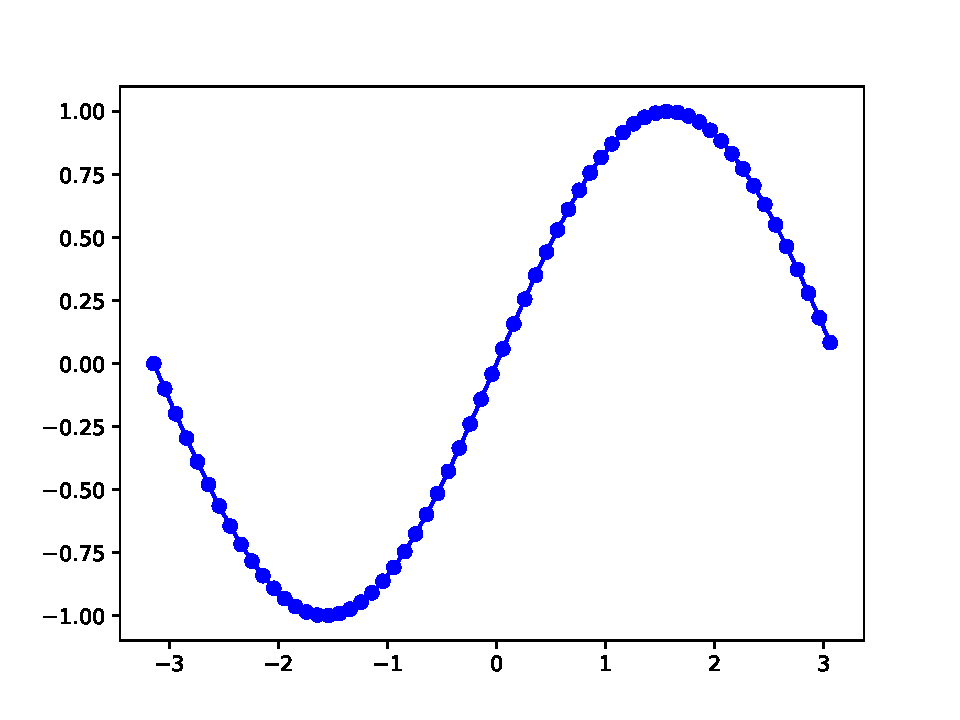
\includegraphics[scale=0.7]{fig/sinx.pdf}
    \caption{ソースコード\ref{matplot1}の出力結果}
    \label{fig:sinx}
\end{figure}

\begin{table}[H]
    \centering
    \caption{主な線の種類}
    \begin{tabular}{c|c}
        \hline
        スクリプト上での記号 & 線の種類 \\
        \hline\hline
        \texttt{-} & 実線 \\
        \texttt{--} & 破線 \\
        \texttt{-.} & 一点鎖線 \\
        \texttt{:} & 点線 \\
        \hline
    \end{tabular}
    \label{tab:linestyle}
\end{table}

\begin{table}[H]
    \centering
    \caption{主なマーカーの種類}
    \begin{tabular}{c|c}
        \hline
        スクリプト上での記号 & 線の種類\\
        \hline\hline
        \texttt{.} & 点 \\
        \texttt{,} & ピクセル \\
        \texttt{o} & 丸 \\
        \texttt{\^} & 三角 \\
        \texttt{v} & 下三角 \\
        \texttt{<} & 左三角 \\
        \texttt{>} & 右三角 \\
        \texttt{s} & 四角 \\
        \texttt{d} & 菱形 \\
        \texttt{+} & $+$ \\
        \texttt{x} & $\times$ \\
        \hline
    \end{tabular}
    \label{tab:marker}
\end{table}

\begin{table}[H]
    \centering
    \caption{主な色の種類}
    \begin{tabular}{c|c}
        \hline
        スクリプト上での記号 & 色\\
        \hline\hline
        \texttt{r} & 赤 \\
        \texttt{g} & 緑 \\
        \texttt{b} & 青 \\
        \texttt{c} & シアン \\
        \texttt{m} & マゼンタ \\
        \texttt{y} & 黄 \\
        \texttt{k} & 黒 \\
        \texttt{w} & 白 \\
        \hline
    \end{tabular}
    \label{tab:color}
\end{table}

なお，matplotlibによる作図では\LaTeX を使うことができる．
ソースコード\ref{matplot1}に対して，\LaTeX の記法に従って軸のラベルを入れるようにしたのがソースコード\ref{matplot2}である．
\texttt{r"..."}と書くことにより，その中で\LaTeX の記法を使うことができる．
\footnote{
\texttt{r"..."}の\texttt{r}はraw stringに由来し，バックスラッシュなどの特殊文字を生の文字列として取り扱う．
}
ソースコード\ref{matplot2}の出力結果を図\ref{fig:sinx_latex}に示す．

\begin{lstlisting}[caption=matplotlibで\LaTeX の記法を使う,label=matplot2]
import matplotlib.pyplot as plt
import numpy as np

plt.rc('text', usetex=True)
plt.rc('font', family='serif')
 
x = np.arange(-np.pi, np.pi, 0.1)
y = np.sin(x)

plt.title(r"Graph Title")
plt.xlabel(r"$x$")
plt.ylabel(r"$\sin x$")
plt.plot(x, y, "-ob")
 
plt.savefig("sinx_latex.pdf")
\end{lstlisting}

\begin{figure}[H]
    \centering
    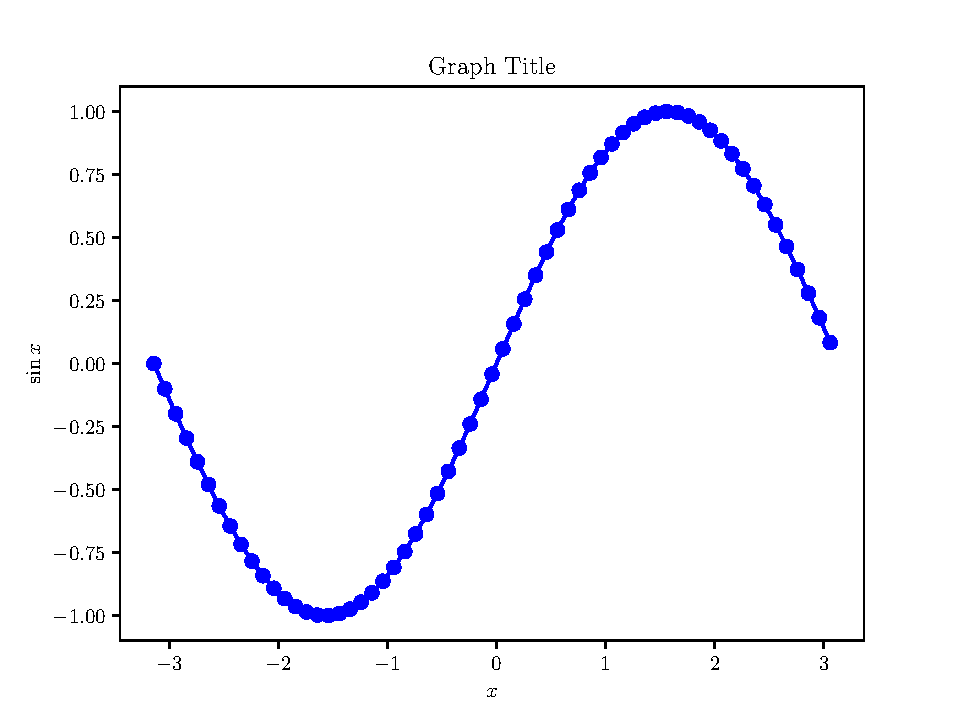
\includegraphics[scale=0.7]{fig/sinx_latex.pdf}
    \caption{ソースコード\ref{matplot2}の出力結果}
    \label{fig:sinx_latex}
\end{figure}

さらに，\texttt{f"..."}を使うことで，Pythonの変数を埋め込むことができる．
\footnote{
\texttt{f"..."}の\texttt{f}はformatted strings literalsに由来し, Pythonの\texttt{format}メソッドを使いやすくしたもの．
}
先ほどの\texttt{r"..."}と組み合わせて\texttt{rf"..."}と書けば, \LaTeX 記法の使用と変数埋め込みの両方に対応できる．
ソースコード\ref{matplot3}とその出力結果\ref{fig:poly_abcd}を見て欲しい．

\begin{lstlisting}[caption=matplotlibでのPython変数の埋め込み,label=matplot3]
import matplotlib.pyplot as plt
import numpy as np

plt.rc('text', usetex=True)
plt.rc('font', family='serif')

a = 2
b = -1
c = -5
d = 3
 
x = np.arange(-np.pi, np.pi, 0.1)
y = a*x*x*x + b*x*x +c*x + d

plt.title(rf"$a = {a}, b = {b}, c = {c}, d = {d}$")
plt.xlabel(rf"$x$")
plt.ylabel(rf"$ax^3+bx^2+cx+d$")
plt.plot(x, y, "-ob")
 
plt.savefig("poly_abcd.pdf")
\end{lstlisting}

Python変数の埋め込みを応用して, 出力ファイル名に入力パラメタの情報を埋め込むこともできる．例えば, ソースコード\ref{matplot3}の20行目を
\texttt{plt.savefig(f"poly\_a\{a\}\allowbreak
b\{b\}\allowbreak c\{c\}\allowbreak d\{d\}.pdf")}
と変更すれば，
「\texttt{poly\_a2b-1c-5d3.pdf}」という名前で図が保存される．
入力パラメタに応じて出力ファイル名が自動的に変わるため，不用意な図の上書きを防止できるだろう．

\begin{figure}[H]
    \centering
    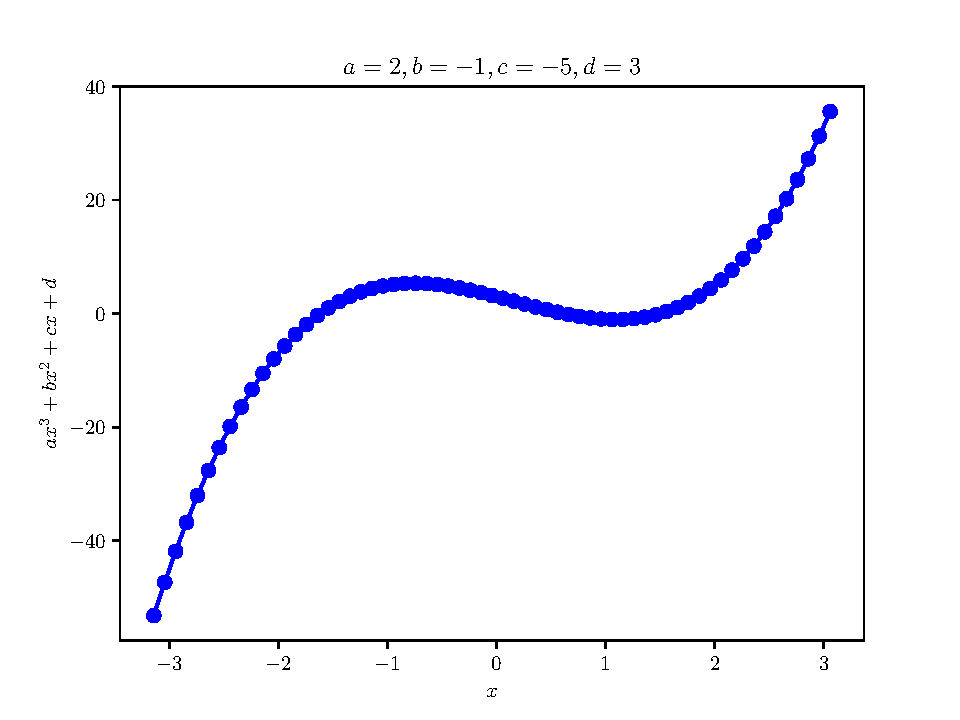
\includegraphics[scale=0.7]{fig/poly_abcd.pdf}
    \caption{ソースコード\ref{matplot3}の出力結果}
    \label{fig:poly_abcd}
\end{figure}

\section{仮想環境}

Pythonでは，プロジェクトごとに独立した実行環境を作成することができる．このような環境を\textbf{仮想環境（virtual environment）}と呼ぶ．仮想環境を利用すると，プロジェクトごとに使用するパッケージやそのバージョンを個別に管理することができる．例えば，あるプログラムでは古いバージョンのNumpyが必要である一方，別のプログラムでは新しいバージョンが必要になる，といった場合があり得る．仮想環境を利用すれば，それぞれの環境に異なるバージョンのNumPyをインストールできるため，互いに影響を与えることなくプログラムを実行できる．

Pythonには，仮想環境を作成するための\texttt{venv}という機能が標準で用意されている．例えば，以下のコマンドを実行すると，\texttt{myenv}という名前の仮想環境を作成できる．

\begin{lstlisting}[language=bash]
python3 -m venv myenv
\end{lstlisting}

LinuxやmacOSでは，作成した仮想環境を以下のように有効化する．
\begin{lstlisting}
source myenv/bin/activate
\end{lstlisting}

仮想環境が有効な状態で，
\begin{lstlisting}[language=bash]
pip install numpy matplotlib
\end{lstlisting}
などを実行すると，これらのパッケージは現在の仮想環境にインストールされる．仮想環境の使用を終了する場合には，

\begin{lstlisting}[language=bash]
deactivate
\end{lstlisting}
を実行する．

初学者のうちは仮想環境を強く意識する必要はないが，複数のプログラムを開発したり，長期間にわたって研究や開発を行ったりする場合には，仮想環境を用いて実行環境を管理することが重要になる．


\end{document}
